\section{Lasso Regression} 

  The Lasso approximates the best subset regression by using a convex relaxation. In particular, the norm $||\beta||_0$ is not convex, but the L1 norm $||\beta||_1$ is. Therefore, we want relax our constraint equation as such: 
  \begin{equation}
    \argmin_{||\beta||_0 \leq L} R(\beta) \mapsto \argmin_{||\beta||_1 \leq L} R(\beta)
  \end{equation}
  This gives us a convex problem, which we can then solve. In fact, it turns out that optimizing the risk given the L1 restriction on the norm is equivalent to minimizing the risk plus a L1 penalty, as this is the Lagrangian form of the original equation (this is in convex optimization). Therefore, there exists a pair $(L, \lambda)$ for which the two problems are equivalent 
  \begin{equation}
    \argmin_{||\beta||_1 \leq L} R(\beta) = \argmin_{\beta} R(\beta) + \lambda ||\beta||_1
  \end{equation}

  Optimizing this gives us a sparse solution. That is, for large enough $\lambda$, many of the components of $\hat{\beta}$ are $0$. 

  \begin{definition}[LASSO Regression]
    \textbf{Lasso regression} takes a linear regression model and minimizes the constrained loss 
    \begin{equation}
      L(\beta, x, y) = (y - \beta^T x)^2 + \lambda \|\beta\|_1
    \end{equation}
    where we penalize according to the L1 norm of the coefficients. 
  \end{definition}

  \begin{theorem}[Risk]
    The risk is 
    \begin{equation}
      R (\beta) = \mathbb{E}_{x, y} \left[ (y - \beta^T x)^2 + \lambda \|\beta\|_1 \right]
    \end{equation}
    The empirical risk is 
    \begin{equation}
      \hat{R} (\beta) = \frac{1}{n} \sum_{i=1}^n (y^{(i)} - \beta^T x^{(i)})^2 + \lambda \|\beta\|_1
    \end{equation}
  \end{theorem}

  Unfortunately, there is no closed form of this best estimator, so we must numerically optimize it. 

\subsection{Sparsity}

  We mentioned sparsity as a main motivation behind the Lasso, but let's formalize this treatment. To gain some intuition, take a look at the example below. 

  \begin{example}[Comparison of $L^0, L^1, L^2$ Norms]
    Let us take the two vectors 
    \begin{align}
      a = \bigg( \frac{1}{\sqrt{d}}, \ldots, \frac{1}{\sqrt{d}} \bigg), \qquad b = ( 1, 0, \ldots, 0)
    \end{align}
    Then the L0, L1, and L2 norms of $a$ are $d, \sqrt{d}, 1$ and those of $b$ are $1, 1, 1$. We want to choose a norm that capture the sparsity of $b$ and distinguishes it from $b$., The L0 norm clearly does this, but the L2 norm does not. The L1 norm is a good compromise between the two. 
  \end{example}

  Now let's establish this fact. 

  \begin{theorem}[Sparse Estimators in Lasso]
    
  \end{theorem}
  \begin{proof}
    
  \end{proof}

  The classical intuition for this is the figure below, where the equipotential lines have ``corners.'' In fact for any $0 < p < 1$, there are also corners, but the problem with using these p-norms is that they are not convex. 

  \begin{figure}[H]
    \centering 
    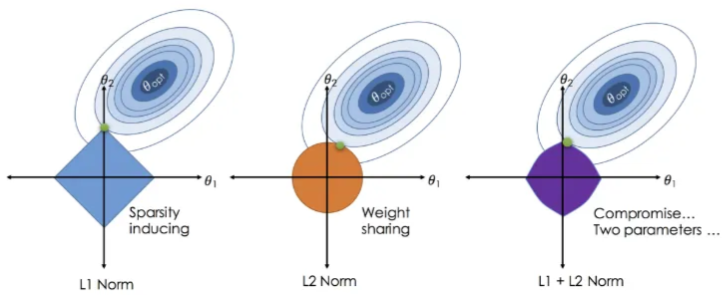
\includegraphics[scale=0.5]{img/regularizers.png}
    \caption{The ridge regularizer draws equipotential circles in our parameter space. The lasso draws a diamond, which tends to give a sparser solution since the loss is most likely to ``touch'' the corners of the contour plots of the regularizer. The elastic net is a linear combination of the ridge and lasso regularizers.} 
    \label{fig:regularizers_visual}
  \end{figure}

\subsection{Bias Variance Tradeoff}

\subsection{Concentration Bounds}

  There are 3 measures we want to talk about: sparsistency, consistency, and risk consistency. 

  \begin{theorem}[Sparsistency: Wainwright 2006]
    Let $\beta = (\beta_1, \ldots, \beta_s, 0, \ldots, 0)$ and decompose the design matrix as $X = (X_S \; X_{S^c})$ where $S = \{1, \ldots, s\}$. Let $\beta_S = (\beta_1, \ldots, \beta_s)$. Suppose that:
    \begin{enumerate}
      \item The true model is linear.
      
      \item The design matrix satisfies
      \begin{equation}
        \|X_S^c X_S (X_S^T X_S)^{-1}\|_{\infty} \leq 1 - \epsilon \quad \text{for some } 0 < \epsilon \leq 1. 
      \end{equation}
      
      \item $\phi_n(d_n) > 0$.
      
      \item The $\epsilon_i$ are Normal.
      
      \item $\lambda_n$ satisfies
      \begin{equation}
        \frac{n\lambda_n^2}{\log(d_n - s_n)} \to \infty
      \end{equation}
      and
      \begin{equation}
        \frac{1}{\min_{1 \leq j \leq s_n} |\beta_j|} \left( \sqrt{\frac{\log s_n}{n}} + \lambda_n \left\| \left( \frac{1}{n} X^T X \right)^{-1} \right\|_{\infty} \right) \to 0. 
      \end{equation}
    \end{enumerate}

    Then the lasso is sparsistent, meaning that $P(\text{support}(\hat{\beta}) = \text{support}(\beta)) \to 1$ where $\text{support}(\beta) = \{j : \beta(j) \neq 0\}$.
  \end{theorem}

  \begin{theorem}[Consistency: Meinshausen and Yu 2006]
    Assume that
    \begin{enumerate}
      \item The true regression function is linear.
      
      \item The columns of $X$ have norm $n$ and the covariates are bounded.
      
      \item $\mathbb{E}(\exp |\epsilon_i|) < \infty$ and $\mathbb{E}(\epsilon_i^2) = \sigma^2 < \infty$.
      
      \item $\mathbb{E}(Y_i^2) \leq \sigma_i^2 < \infty$.
      
      \item $0 < \phi_n(k_n) \leq \Phi_n(k_n) < \infty$ for $k_n = \min\{n, d_n\}$.
      
      \item $\liminf_{n \to \infty} \phi_n(s_n \log n) > 0$ where $s_n = \|\beta_n\|_0$.
    \end{enumerate}

    Then
    \begin{equation}
      \|\hat{\beta}_n - \beta_n\|^2 = O_P \left( \frac{\log n}{\phi_n^2(s_n \log n)} \right) + O \left( \frac{1}{\log n} \right) 
    \end{equation}

    If
    \begin{equation}
      s_n \log d_n \left( \frac{\log n}{n} \right) \to 0 
    \end{equation}

    and
    \begin{equation}
      \lambda_n = \sqrt{\frac{\sigma_n^2 \Phi_n(\min\{n, d_n\})n^2}{s_n \log n}} 
    \end{equation}

    then $\|\hat{\beta}_n - \beta_n\|^2 \xrightarrow{P} 0$.

    Once again, the conditions of this theorem are very strong. They are not checkable and they are unlikely to ever be true in practice.
  \end{theorem}

  Theoretically and practically, these two results are important, but it has the unrealistic assumption that the true model is both linear, which is not checkable and unlikely to be every true in practice. Because of the linearity, we also have the strong assumption of multicollinearity, which can be a problem if it is high (though not perfect). For example, if for some reason---by chance or by some other factor---that covariate $x_1$ and $x_{12}$ were correlated, then we won't be able to separate them. 

  The next concentration result on bounded covariates does not assume anything except for iid data (distribution free) and essentially proves why Lasso regression works in high dimensions. 

  \begin{theorem}[Concentration of Lasso]
    Given $(X, Y)$, assume that $|Y| \leq B$ and $\max_j |X_j| \leq B$. Let 
    \begin{equation}
      \beta^\ast = \argmin_{||\beta||_1 \leq L} R(\beta)
    \end{equation}
    be the best sparse linear predictor in the L1 sense, where $R(\beta) = \mathbb{E}[ (Y - \beta^T X)^2]$. Let our lasso estimator be 
    \begin{equation}
      \hat{\beta} = \argmin_{||\beta||_1 \leq L} \hat{r}(\beta) = \argmin_{||\beta||_1 \leq L} \frac{1}{n} \sum_{i=1}^n (Y_i - \beta^T X_i)^2
    \end{equation}
    which minimizes the empirical risk. Then, with probability at least $1 - \delta$, 
    \begin{equation}
      r(\hat{\beta}) \leq R(\beta^\ast) + \sqrt{\frac{16(L+1)^4 B^2}{n} \log \bigg( \frac{\sqrt{2} d}{\sqrt{\delta}} \bigg)} 
    \end{equation}
  \end{theorem}
  \begin{proof}
    Let $Z = (Y, X)$ and $Z_i = (Y_i, X_i)$. Define $\gamma \equiv \gamma(\beta) = (-1, \beta)$. Then
    \begin{equation}
      r(\beta) = \mathbb{E}(Y - \beta^T X)^2 = \gamma^T \Lambda \gamma
    \end{equation}
    where $\Lambda = \mathbb{E}[ZZ^T]$. Note that $\|\gamma\|_1 = \|\beta\|_1 + 1$. Let $\mathcal{B} = \{\beta : \|\beta\|_1 \leq L\}$. The training error is
    \begin{equation}
      \hat{r}(\beta) = \frac{1}{n} \sum_{i=1}^n (Y_i - X_i^T \beta)^2 = \gamma^T \hat{\Lambda} \gamma
    \end{equation}
    where $\hat{\Lambda} = \frac{1}{n} \sum_{i=1}^n Z_i Z_i^T$. For any $\beta \in \mathcal{B}$,
    \begin{align}
      |\hat{r}(\beta) - r(\beta)| &= |\gamma^T (\hat{\Lambda} - \Lambda) \gamma| \\
      &\leq \sum_{j,k} |\gamma(j)| |\gamma(k)| |\hat{\Lambda}(j,k) - \Lambda(j,k)| \leq \|\gamma\|_1^2 \delta_n \\
      &\leq (L + 1)^2 \Delta_n
    \end{align}
    where
    \begin{equation}
      \Delta_n = \max_{j,k} |\hat{\Lambda}(j,k) - \Lambda(j,k)|.
    \end{equation}
    So,
    \begin{equation}
      r(\hat{\beta}) \leq \hat{r}(\hat{\beta}) + (L + 1)^2 \Delta_n \leq \hat{r}(\beta_*) + (L + 1)^2 \Delta_n \leq r(\beta_*) + 2(L + 1)^2 \Delta_n.
    \end{equation}
    Note that $|Z(j)Z(k)| \leq B^2 < \infty$. By Hoeffding's inequality,
    \begin{equation}
      \mathbb{P}(\Delta_n(j,k) \geq \epsilon) \leq 2e^{-n\epsilon^2/(2B^2)}
    \end{equation}
    and so, by the union bound,
    \begin{equation}
      \mathbb{P}(\Delta_n \geq \epsilon) \leq 2d^2 e^{-n\epsilon^2/(2B^2)} = \delta
    \end{equation}
    if we choose $\epsilon = \sqrt{(4B^2/n) \log \left( \frac{\sqrt{2}d}{\sqrt{\delta}} \right)}$. Hence,
    \begin{equation}
      r(\hat{\beta}) \leq r(\beta_*) + \sqrt{\frac{16(L + 1)^4 B^2}{n} \log \left( \frac{\sqrt{2}d}{\sqrt{\delta}} \right)}
    \end{equation}
    with probability at least $1 - \delta$. $\square$
  \end{proof}

  Note that $\epsilon \approx \sqrt{\log{d}/n}$, and since it scales nicely with $d$, this is what allows us to do sparse regression in high dimensions. 

\subsection{Optimization}

  Soft Thresholding and Proximal Gradient Descent

  \begin{code}[MWS of Lasso Regression in scikit-learn]
    \noindent\begin{minipage}{.6\textwidth}
    \begin{lstlisting}[]{Code}
      from sklearn.linear_model import Lasso

      X = np.random.randn(10, 5) 
      y = np.random.randn(10)
      # regularization parameter
      model = Lasso(alpha=1e-1)  
      model.fit(X, y) 
      print(model.score(X, y))  
      print(model.intercept_)
      print(model.coef_) 
      print(model.predict(np.array([[1, 2, 3, 4, 5]]))) 
    \end{lstlisting}
    \end{minipage}
    \hfill
    \begin{minipage}{.39\textwidth}
    \begin{lstlisting}[]{Output}
      0.47590269719236045
      -0.8861298412689853
      [0.         0.10767647 0.24172197 0.7427863  0.        ]
      [3.02553422]
      .
      .
      .
      .
      .
    \end{lstlisting}
    \end{minipage}
  \end{code}

\subsection{Sparse Minimax Estimators}

  Now let's talk about the big weakness of sparse estimators. Intuitively, sparsity isn't really smooth (a variable is either $0$ or not $0$), and this is at a high-level a bad thing. In fact, in practice sparse estimators may not work well. They are terrible minimax estimators. 

  Say that $\hat{\beta}$ is weakly sparsistent if, for every $\beta$,
  \begin{equation}
    P_{\beta}(I(\hat{\beta}_j = 0) \leq I(\beta_j = 0) \text{ for all } j) \to 1
  \end{equation}
  as $n \to \infty$. In particular, if $\hat{\beta}_n$ is sparsistent, then it is weakly sparsistent. Suppose that $d$ is fixed. Then the least squares estimator $\hat{\beta}_n$ is minimax and satisfies
  \begin{equation}
    \sup_{\beta} E_{\beta}(n\|\hat{\beta}_n - \beta\|^2) = O(1). 
  \end{equation}

  But sparsistent estimators have much larger risk:

  \begin{theorem}[Leeb and Potscher, 2007]
    Given a regression model $y = \beta^T x + \epsilon$, suppose that the following conditions hold:
    \begin{enumerate}
      \item $d$ is fixed.
      
      \item The covariates are nonstochastic and $n^{-1}X^T X \to Q$ for some positive definite matrix $Q$.
      
      \item The errors $\epsilon_i$ are independent with mean $0$, finite variance $\sigma^2$ and have a density $f$ satisfying
      \begin{equation}
        0 < \int \left( \frac{f'(x)}{f(x)} \right)^2 f(x) dx < \infty.
      \end{equation}
    \end{enumerate}
    If $\hat{\beta}$ is weakly sparsistent then
    \begin{equation}
      \sup_{\beta} E_{\beta}(n\|\hat{\beta}_n - \beta\|^2) \to \infty. 
    \end{equation}
    More generally, if $L$ is any nonnegative loss function then
    \begin{equation}
      \sup_{\beta} E_{\beta}(L(n^{1/2}(\hat{\beta}_n - \beta))) \to \sup_s L(s). 
    \end{equation}
  \end{theorem}
  \begin{proof}
    Choose any $s \in \mathbb{R}^d$ and let $\beta_n = -s/\sqrt{n}$. Then,
    \begin{align}
      \sup_{\beta} E_{\beta}(L(n^{1/2}(\hat{\beta} - \beta))) &\geq E_{\beta_n}(L(n^{1/2}(\hat{\beta} - \beta))) \geq E_{\beta_n}(L(n^{1/2}(\hat{\beta} - \beta))) I(\hat{\beta} = 0) \\
      &= L(-\sqrt{n}\beta_n) P_{\beta_n}(\hat{\beta} = 0) = L(s) P_{\beta_n}(\hat{\beta} = 0).
    \end{align}
    Now, $P_0(\hat{\beta} = 0) \to 1$ by assumption. It can be shown that we also have $P_{\beta_n}(\hat{\beta} = 0) \to 1.^2$ Hence, with probability tending to $1$,
    \begin{equation}
      \sup_{\beta} E_{\beta}(L(n^{1/2}(\hat{\beta} - \beta))) \geq L(s).
    \end{equation}
    Since $s$ was arbitrary the result follows. $\square$
  \end{proof}
